% +--------------------------------------------------------------------+
% | Sample Chapter 1
% |
% | This file provides examples of how to
% | - insert a figure with a caption
% | - construct a table with a caption
% | - create subsections within the chapter
% | - insert a reference to a Figure or Table
% | - make a citation
% +--------------------------------------------------------------------+

\cleardoublepage

% +--------------------------------------------------------------------+
% | Replace "Chapter Title" below with the title of your chapter.
% | LaTeX will automatically number the chapters.
% +--------------------------------------------------------------------+

\chapter{Introduction}
\label{makereference1}
\section{Motivation}
\section{Objective}












In this chapter there examples of various features you may want to
incorporate into your document. Here's an example of a figure
inserted into the text:

\begin{figure}[htb]%t=top, b=bottom, h=here

    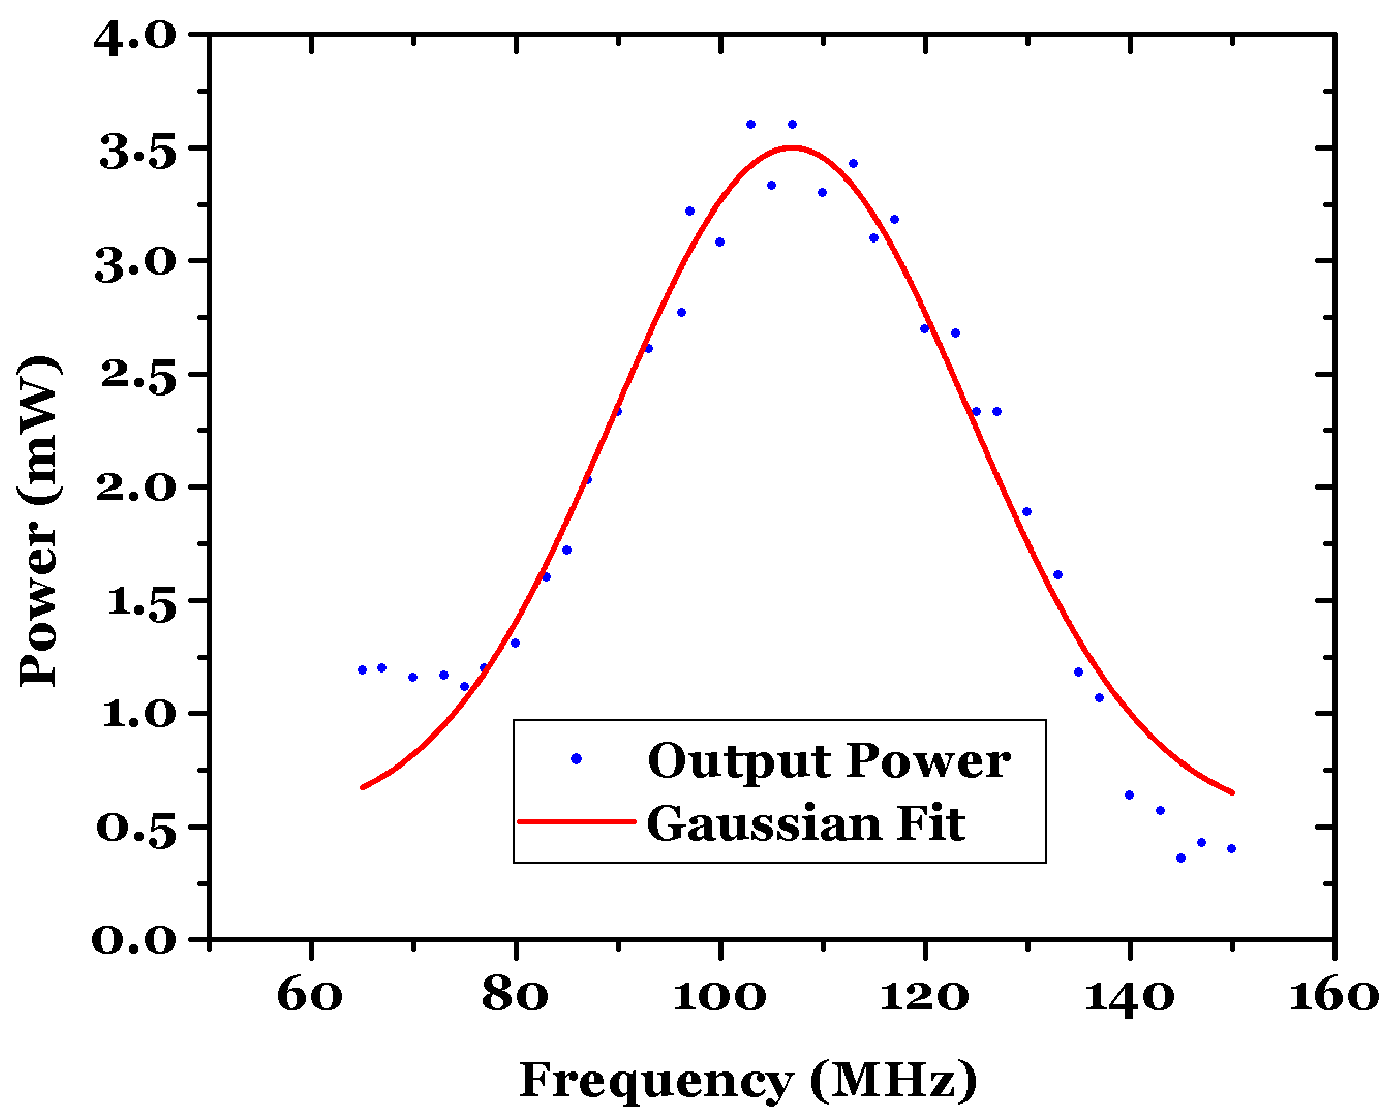
\includegraphics[height=2.5in]{tex/figures/graph.png}

    \caption[Optional: Short caption to appear in List of
    Figures]{Full caption to appear below the Figure}

    \label{figure1}
\end{figure}

% +--------------------------------------------------------------------+
% |To create cross-references to figures, tables and segments
% |of text, LaTeX provides the following commands:
% |   \label{marker}
% |   \ref{marker}
% |   \pageref{marker}
% | where {marker} is a unique identifier.
% |
% | In the line above, we use \label{figure1} to mark a location
% | we wish to refer to later.  LATEX replaces \ref by the number of
% | the chapter, section, subsection, figure, or table after which the
% | corresponding \label command was issued. \pageref prints the page
% | number of the page where the \label command occurred.
% |
% +--------------------------------------------------------------------+

See the file chapter1.tex for examples of the commands used to
insert a figure or table, add a caption, etc.  Here is an example of
a table:

\begin{table}[ht]

% +--------------------------------------------------------------------+
% | We include the command \begin{center} to center the table
% | horizontally on the page.  Note use of the command \end{center}
% | to turn off centering after the table is defined.
% +--------------------------------------------------------------------+
    \begin{center}

% +--------------------------------------------------------------------+
% | The table is created with this command
% |
% | \begin{tabular}[pos]{table spec}
% |
% | The "pos" argument specifies the vertical position of the table
% | relative to the baseline of the surrounding text.  Use t, b, or c
% | to specify alignment at the top, bottom, or center.
% |
% | The "table spec" command defines the format of the table
% |   l for a column of left-aligned text
% |   r for a column of right-aligned text
% |   c for centered text
% |   p{width} for a column containing justified text with line breaks
% |   | for a vertical line
% |
% |  In this example, the caption is made to appear above the table
% |  by positioning the \caption command before the \begin{tabular
% |  command. To position the caption below the table, insert the
% |  \caption command after the \end{tabular} command.
% +--------------------------------------------------------------------+
    \caption{Caption to appear above the table}
    \begin{tabular}[c]{|c|c|c|}
        \hline
        Column 1 Heading & Column 2 Heading & Column 3 Heading \\
        \hline
        Col 1 Row 1 & Col 2 Row 1 & Col 3 Row 1\\
        Col 1 Row 2 & Col 2 Row 2 & Col 3 Row 2\\
        Col 1 Row 3 & Col 2 Row 3 & Col 3 Row 3\\
        \hline
    \end{tabular}

    \label{table1}
   \end{center}
\end{table}



% +--------------------------------------------------------------------+
% | Replace \section headings below with the title of your
% | subsections.  LaTeX will automatically number the subsections 1.1,
% | 1.2, 1.3, etc.
% +--------------------------------------------------------------------+

\section{Making References to Figures or Tables}
\label{makereference1.1}

It is possible to create cross-references and hyperlinks to items or
sections within your paper.  For example, here is a reference to
Fig.~\ref{figure1} mentioned at the beginning of this chapter and a
reference to the Table~\ref{table1}.

\section{Making a Reference to a Chapter Subsection}
\label{makereference1.2}

In this section, we refer back to text mentioned in
Section~\ref{makereference1.1} on page~\pageref{makereference1.1}.

\section{Making a Citation}
\label{makereference1.3}

%Here's an example of a citation to a single
%work.~\citep{CT:Weiner:1999} It's also possible to make multiple
%citations.~\citep{CT:Phillips:1985, ARP:Loy:1974}
%
%This template uses BibTeX to manage and format citations.  BibTeX is
%not the only way to create a bibliography within LaTeX, but it's
%generally considered to be the best option for long documents like a
%thesis or dissertation.~\citep{CT:Gould:1988}  There are a few more
%sample citations in this paragraph so you can see examples of how
%in-text references are made and how the bibliography is
%formatted.~\citep{ARP:Melinger:1991} See the file "BibTeX Guide.pdf"
%for information on how to use BibTeX.
